\documentclass[10pt,a4paper]{article}

\usepackage[a4paper,top=10.5mm,bottom=10.5mm,left=12mm,right=12mm]{geometry}
\usepackage[T1]{fontenc}
\usepackage[default]{lato}
\usepackage{graphicx}
\usepackage{xcolor}
\usepackage{microtype}
\usepackage{hyperref}
\usepackage{enumitem}
\usepackage{tabularx}
\usepackage{array}
\usepackage{ragged2e}
\usepackage{setspace}
\usepackage{fancyhdr}
\usepackage{lastpage}
\usepackage{calc}

\definecolor{Navy}{HTML}{17324D}
\definecolor{Teal}{HTML}{0F7182}
\definecolor{Ink}{HTML}{17202A}
\definecolor{Muted}{HTML}{5D6773}
\definecolor{Rule}{HTML}{D6DEE5}
\definecolor{Soft}{HTML}{EEF4F7}
\definecolor{SoftBlue}{HTML}{E7F1F4}

\hypersetup{
  colorlinks=true,
  urlcolor=Teal,
  linkcolor=Navy,
  pdfauthor={Jia-Hao Ji},
  pdftitle={Jia-Hao Ji - One-Page Research Resume},
  pdfsubject={Biomedical AI, spatial omics, and multi-agent reasoning},
  pdfkeywords={biomedical AI, agentic AI, spatial omics, multi-agent systems, neuroscience}
}
\urlstyle{same}

\pagestyle{empty}
\setlength{\parindent}{0pt}
\setlength{\parskip}{0pt}
\setstretch{1.00}
\emergencystretch=1em
\hyphenpenalty=10000
\exhyphenpenalty=10000
\graphicspath{{./}{public/}{../public/}}

\newcommand{\sectiontitle}[1]{%
  \vspace{0.55em}%
  {\fontsize{10.7}{11.5}\selectfont\bfseries\color{Navy}#1}\par
  \vspace{-0.22em}\color{Rule}\rule{\linewidth}{0.45pt}\color{Ink}\vspace{0.27em}
}
\newcommand{\sideheading}[1]{%
  \vspace{0.45em}%
  {\fontsize{9.2}{10}\selectfont\bfseries\color{Navy}\MakeUppercase{#1}}\par
  \vspace{0.12em}\color{Teal}\rule{\linewidth}{0.7pt}\color{Ink}\vspace{0.25em}
}
\newcommand{\smallmeta}[1]{{\fontsize{7.8}{9.1}\selectfont\color{Muted}#1}}
\newcommand{\bodytext}[1]{{\fontsize{8.35}{9.8}\selectfont\RaggedRight #1}}
\newcommand{\pubentry}[4]{%
  {\fontsize{8.75}{10.1}\selectfont\bfseries\color{Ink}\RaggedRight #1}\par
  \smallmeta{#2}\par
  \vspace{0.08em}
  {\fontsize{8.15}{9.55}\selectfont\RaggedRight #3}\par
  \vspace{0.06em}
  {\fontsize{7.8}{9.1}\selectfont\bfseries\color{Teal}#4}\par
  \vspace{0.38em}
}
\newcommand{\role}[3]{%
  \begin{tabularx}{\linewidth}{@{}>{\RaggedRight\arraybackslash}X>{\RaggedLeft\arraybackslash}p{24mm}@{}}
    {\fontsize{8.65}{9.9}\selectfont\bfseries\color{Ink}#1} & {\fontsize{7.8}{9}\selectfont\color{Muted}#3}\\[-0.08em]
    {\fontsize{8.05}{9.2}\selectfont\color{Teal}#2} &
  \end{tabularx}\vspace{0.03em}
}
\newenvironment{compactitems}{%
  \begin{itemize}[leftmargin=1.05em,itemsep=0.09em,topsep=0.08em,parsep=0pt,partopsep=0pt,label=\textcolor{Teal}{\raisebox{0.18ex}{\tiny\textbullet}}]
  \fontsize{8.05}{9.45}\selectfont\RaggedRight
}{\end{itemize}}
\newcommand{\sidebaritem}[2]{%
  {\fontsize{8.15}{9.35}\selectfont\bfseries\color{Ink}\RaggedRight #1}\par
  {\fontsize{7.8}{9.1}\selectfont\color{Muted}\RaggedRight #2}\par\vspace{0.31em}
}
\newcommand{\skillline}[2]{%
  {\fontsize{7.85}{9.2}\selectfont\bfseries\color{Navy}\RaggedRight #1}\par
  {\fontsize{7.65}{9.05}\selectfont\color{Ink}\RaggedRight #2}\par\vspace{0.28em}
}
\newcommand{\tag}[1]{\colorbox{SoftBlue}{\strut\hspace{0.28em}\fontsize{7.2}{8.2}\selectfont\bfseries\color{Navy}#1\hspace{0.28em}}}

\begin{document}
\fontsize{8.35}{9.8}\selectfont

% Header
\begin{tabularx}{\textwidth}{@{}X>{\RaggedLeft\arraybackslash}p{31mm}@{}}
  \begin{minipage}[t]{\linewidth}
    \vspace{0pt}
    {\fontsize{25.5}{27}\selectfont\bfseries\color{Ink}Jia-Hao (Jay) Ji}\par
    \vspace{0.18em}
    {\fontsize{11.2}{12.4}\selectfont\bfseries\color{Navy}M.D. Candidate \textbar{} AI Researcher \textbar{} Physician-Scientist in Training}\par
    \vspace{0.45em}
    {\fontsize{8.6}{10}\selectfont\color{Muted}\RaggedRight
      Building reliable agentic and multimodal AI systems for biomedical discovery, with current work in spatial omics, neuroscience, and multi-agent reasoning.
    }\par
    \vspace{0.45em}
    {\fontsize{7.85}{9}\selectfont\color{Muted}
      Shanghai, China \hspace{0.45em}\textcolor{Rule}{\textbullet}\hspace{0.45em}
      \href{mailto:jhji19@fudan.edu.cn}{jhji19@fudan.edu.cn} \hspace{0.45em}\textcolor{Rule}{\textbullet}\hspace{0.45em}
      \href{https://jiahaoblog.com}{jiahaoblog.com} \hspace{0.45em}\textcolor{Rule}{\textbullet}\hspace{0.45em}
      \href{https://github.com/Biogod2020}{GitHub} \hspace{0.45em}\textcolor{Rule}{\textbullet}\hspace{0.45em}
      \href{https://orcid.org/0009-0007-4647-522X}{ORCID}
    }\par
  \end{minipage}
  &
  \begin{minipage}[t]{31mm}
    \vspace{0pt}
    \fcolorbox{Rule}{white}{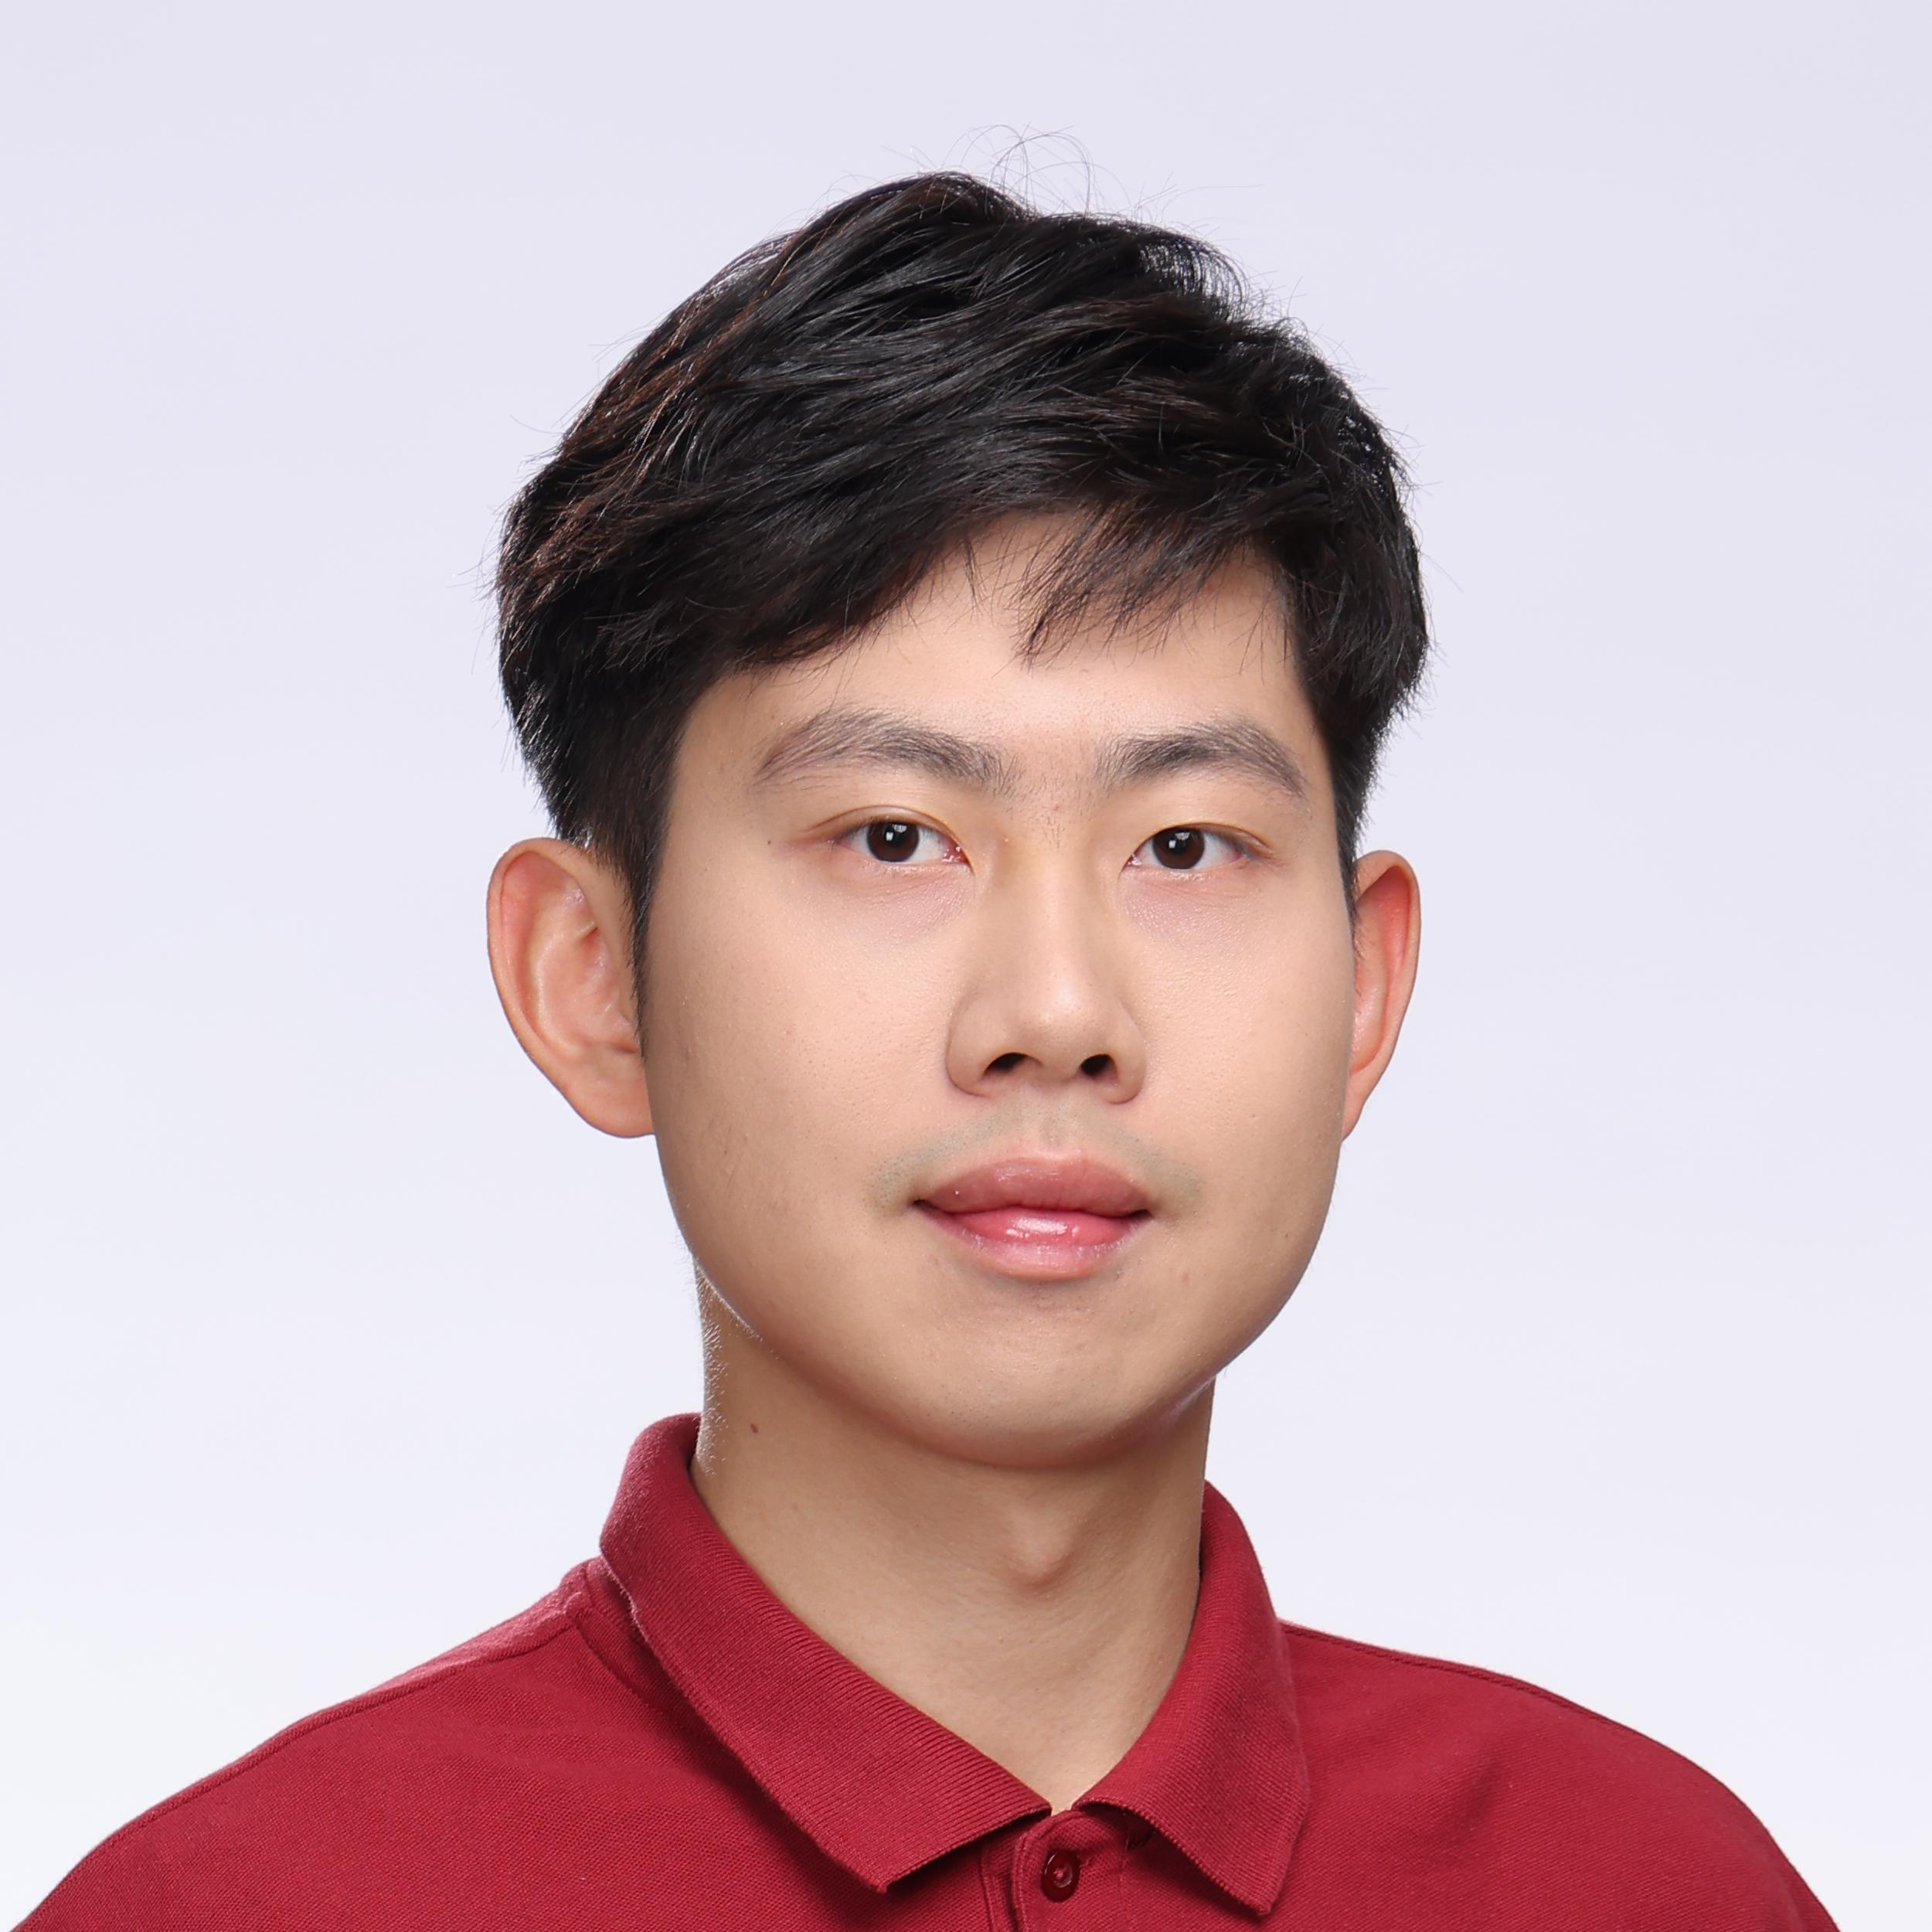
\includegraphics[width=27.5mm,trim=460 465 460 60,clip]{avatar.jpg}}
  \end{minipage}
\end{tabularx}

\vspace{0.42em}
\color{Navy}\rule{\textwidth}{1.7pt}\color{Ink}
\vspace{0.38em}

\tag{AGENTIC AI FOR SCIENCE}\hspace{0.32em}
\tag{SPATIAL OMICS}\hspace{0.32em}
\tag{MULTIMODAL LEARNING}\hspace{0.32em}
\tag{MULTI-AGENT REASONING}\hspace{0.32em}
\tag{NEUROSCIENCE}

\vspace{0.18em}

% Two-column body
\begin{minipage}[t]{0.665\textwidth}
\vspace{0pt}\RaggedRight

\sectiontitle{Selected Research}

\pubentry
{Candidate supply and answer selection shape the value of LLM judging in multi-agent systems}
{\textbf{Jia-Hao Ji} et al. First author. arXiv:2608.25937, 2026. \href{https://arxiv.org/abs/2608.25937}{Paper}}
{Separated candidate generation, answer recognition, and terminal selection across five benchmarks. Correct answers were often generated but lost during consensus.}
{15,336 questions \textbar{} 81,390 candidate-pool replays \textbar{} 63.82\% to 70.82--70.95\% by changing only selection}

\pubentry
{SpatialDataAgent: Autonomous Spatial Omics Data Curation at Decade Scale}
{\textbf{Jia-Hao Ji} et al. First author and lead developer. bioRxiv, 2026. \href{https://doi.org/10.64898/2026.05.27.727615}{DOI}}
{Built an evidence-grounded agentic workflow for recovering, auditing, and standardising fragmented multimodal spatial-omics records.}
{769 paired H\&E--ST datasets \textbar{} 29.2 million spots or cells \textbar{} 6.4-fold expansion over curated baselines}

\pubentry
{Spatiotemporally resolved transcriptome unveils reactive subpallial microglia underlying cholinergic vulnerability in Alzheimer's disease}
{\textbf{Jia-Hao Ji} (co-first author) et al. Manuscript, 2026.}
{Integrated spatial transcriptomics, single-nucleus sequencing, and in situ amyloid pathology to map disease-associated microglial states and cholinergic vulnerability.}
{12.36 million spatial profiles}

\sectiontitle{Research Experience}

\role{Researcher and Project Lead}{Fudan Data-Driven Future Lab \& Institute of Medical Genetics}{Sep 2023 -- Present}
\smallmeta{Advisors: Prof. Jin-Tai Yu and Prof. Zhiyuan Yuan \textbar{} Alzheimer's disease, spatial omics, and biomedical AI}
\begin{compactitems}
  \item Lead computational projects in large-scale spatial-data curation, multimodal tissue registration, and disease-focused analysis of histology and molecular profiles.
  \item Developed transformer and image-registration pipelines aligning whole-slide pathology with spatial transcriptomics; designed auditable agentic workflows with explicit schemas and multi-stage validation.
  \item Investigated LLM-judge reliability and terminal answer selection through controlled candidate-pool replay experiments.
\end{compactitems}

\vspace{0.16em}
\role{Undergraduate Researcher}{Prof. Bin Song's Lab, Fudan University}{Oct 2021 -- Jun 2023}
\begin{compactitems}
  \item Built scRNA-seq pipelines to identify markers relevant to the purity, safety, and therapeutic potential of iPSC-derived dopaminergic progenitor transplantation.
\end{compactitems}

\vspace{0.12em}
\role{Undergraduate Researcher}{Prof. Fei Lan's Lab, Institutes of Biomedical Sciences}{Sep 2019 -- Jul 2021}
\begin{compactitems}
  \item Received wet-lab training in molecular biology, cell culture, DNA methylation, epigenetics, and biochemical assays.
\end{compactitems}

\sectiontitle{Selected Systems}
\bodytext{\textbf{ASSA}: modular agent framework with hierarchical memory, reflection, and skill generation for long-horizon work (\href{https://github.com/Biogod2020/ASSA}{GitHub}). \quad \textbf{Spatial-CLIP}: contrastive vision-language alignment of histopathology with spatial-transcriptomic states (\href{https://github.com/Biogod2020/Spatial-Clip}{GitHub}).}

\end{minipage}
\hfill
\color{Rule}\vrule width 0.45pt\color{Ink}
\hfill
\begin{minipage}[t]{0.295\textwidth}
\vspace{0pt}\RaggedRight

\sideheading{Education}
\sidebaritem{M.D., Eight-Year Clinical Medicine Program}{Shanghai Medical College, Fudan University\\Sep 2019 -- Jun 2027 (expected)}
\sidebaritem{International Exchange Program}{University of California, Los Angeles\\Sep 2021 -- Feb 2022}
\sidebaritem{Clinical Elective, Department of Medicine}{HKU Queen Mary Hospital\\Apr 2025 -- May 2025}

\sideheading{Research Focus}
\skillline{Agentic AI for Science}{Evidence-grounded autonomous systems for scientific data and workflows.}
\skillline{Multimodal Biomedical AI}{Spatial omics, digital pathology, tissue registration, and neurological disease.}
\skillline{Reliable Multi-Agent Reasoning}{Candidate generation, judge reliability, communication, and answer selection.}

\sideheading{Technical Skills}
\skillline{Machine Learning}{PyTorch; transformers; graph neural networks; contrastive learning; vision-language models; LLM agents; multi-agent systems.}
\skillline{Biomedical Data}{Spatial transcriptomics; single-cell RNA-seq; whole-slide imaging; histopathology; computational neuroscience.}
\skillline{Engineering}{Python; R; TypeScript; Linux; Git; HPC; multi-GPU training; parallel API workflows.}

\sideheading{Teaching and Honours}
\bodytext{Invited speaker and workshop instructor on AI-native research workflows for medical students and researchers, Fudan University, 2025.}\par
\vspace{0.34em}
\bodytext{First Prize, China National Biology Olympiad (Guangdong); ranked 9th in Guangdong Province.}\par

\sideheading{Languages}
\bodytext{Mandarin, Cantonese, and Teochew; English (TOEFL 105); Spanish (basic).}

\vfill
{\fontsize{7.2}{8.3}\selectfont\color{Muted}Updated September 2026}

\end{minipage}

\end{document}
